% This is a model template for the solutions in computational science. You can find a very useful documentation for LaTeX in Finnish at ftp://ftp.funet.fi/pub/TeX/CTAN/info/lshort/finnish/ or in English at ftp://ftp.funet.fi/pub/TeX/CTAN/info/lshort/english/. The section List of mathematical symbols in Chapter 3 is especially useful for the typesetting of mathematical formulas.

% Compile the document to PDF by command 'pdflatex model.tex' in the terminal. The command must be run twice for the references in the text to be correct.

\documentclass[a4paper,11pt]{article}
\usepackage[utf8]{inputenc}
% This includes letters such as � and �
\usepackage[T1]{fontenc}
% Use here 'Finnish' for Finnish hyphenation. You may have to compile the code twice after the change. 
\usepackage[english]{babel}
\usepackage{graphicx}
% Some math stuff
\usepackage{amsmath,amsfonts,amssymb,amsbsy,commath,booktabs,hyperref}  
% This is just to include the urls
\usepackage{hyperref}
\usepackage[margin=2cm]{geometry}

\setlength{\parindent}{0mm}
\setlength{\parskip}{1.0\baselineskip}

\usepackage{listings}
\usepackage{color}
\usepackage{pdfpages}

\definecolor{dkgreen}{rgb}{0,0.6,0}
\definecolor{gray}{rgb}{0.5,0.5,0.5}
\definecolor{mauve}{rgb}{0.58,0,0.82}

\lstset{frame=tb,
	language=Python,
	aboveskip=3mm,
	belowskip=3mm,
	showstringspaces=false,
	columns=flexible,
	basicstyle={\tiny\ttfamily},
	numbers=none,
	numberstyle=\tiny\color{gray},
	keywordstyle=\color{blue},
	commentstyle=\color{dkgreen},
	stringstyle=\color{mauve},
	breaklines=true,
	breakatwhitespace=true,
	tabsize=4
}

\begin{document}

\title{Becs-114.1100 Computational Science -- exercise round 6} % Replace the exercise round number
\author{Kunal Ghosh, 546247} % Replace with your name and student number
\maketitle
\section{Solution to Question 4}
\subsection{Determining the natural cubic interpoland S(x) and its Derivative S'(x) from experimental data}\label{prob2a}
\begin{figure}[ht]
	\center
    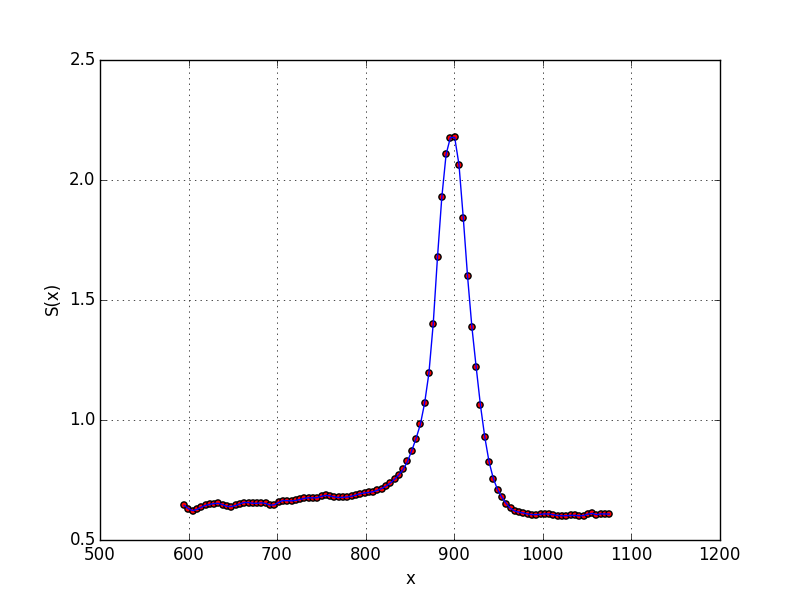
\includegraphics[scale=0.75]{plotS.png}
    \caption{Plot showing the natural cubic interpoland S(X). Values of $S(X_i)$ for $X_i$ in the range of (min(knot values), max(knot values)) are shown as red circles.}
	\label{fig:s}
\end{figure}
\begin{figure}[ht]
	\center
    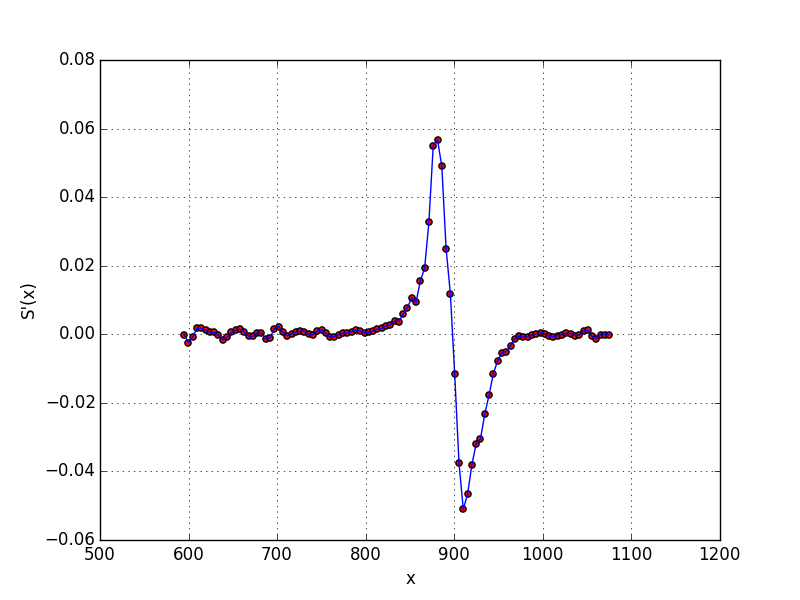
\includegraphics[scale=0.75]{plotS_dash.png}
    \caption{Plot showing the first derivative of the natural cubic interpoland S'(X). Values of $S'(X_i)$ for $X_i$ in the range of (min(knot values), max(knot values)) are shown as red circles.} 
	\label{fig:sdash}
\end{figure}


% \begin{table}[ht]
% \centering
% \label{my-label}
% \begin{tabular}{|c|c|c|}
% \hline
%  \textbf{n}&\textbf{RMS Error}&\textbf{Condition Number}  \\ \hline
%  2&0.73833521&15.0167409881  \\ \hline
%  5&1.02602254&282901.77002 \\ \hline
%  8&1.09505307&7657562245.89 \\ \hline
%  12&1.16783884&5.89342127254e+15 \\ \hline
%  15&2.11656192&1.74359790918e+17 \\ \hline
% \end{tabular}
% \caption{Table showing the values of n and the RMS error after solving the system of linear equations with \textbf{hilbert(n)} as the coefficients.}
% \end{table}
The corresponding python code can be found at \ref{code:problem2a}

\subsection{Determining the natural cubic interpoland S(x) and its Derivative S'(x) from experimental data}\label{prob2b}
\begin{figure}[ht]
	\center
    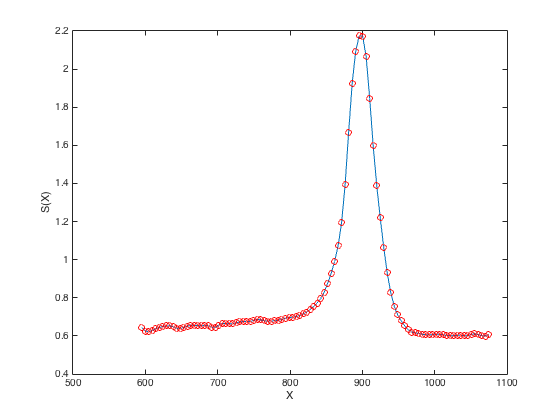
\includegraphics[scale=0.75]{matlabS.png}
    \caption{Plot showing the natural cubic interpoland S(X) as calculated using Matlab. Values of $S(X_i)$ for $X_i$ in the range of (min(knot values), max(knot values)) are shown as red circles.}
	\label{fig:smatlab}
\end{figure}
\begin{figure}[ht]
	\center
    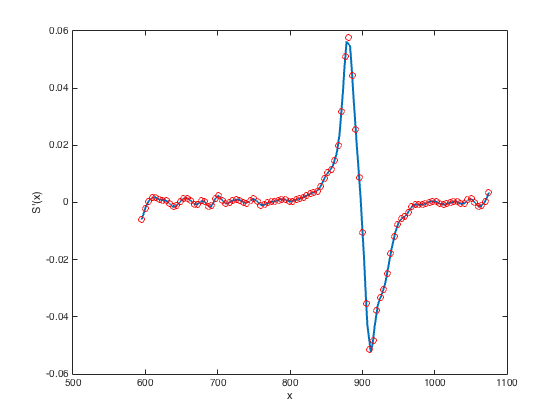
\includegraphics[scale=0.75]{matlabS_dash.png}
    \caption{Plot showing the first derivative of the natural cubic interpoland S'(X) as calculated using Matlab. Values of $S'(X_i)$ for $X_i$ in the range of (min(knot values), max(knot values)) are shown as red circles.} 
	\label{fig:sdash_matlab}
\end{figure}
The corresponding plots created by matlab are much more smoother because matlab implements an additional constraint that the third derivatives of the piecewise polynomials are also equal at the second and the last knots. This are apparently called the "Not-A-Knot" end conditions. This is only done when the length of \textbf{t} and \textbf{y} are same.

Natural splines are a good choice only when the functions have 0 second derivative at the end points. I read it up from here. \url{http://www.mathworks.com/matlabcentral/newsreader/view_thread/172988} would really appreciate some more information about why using the Not-A-Knot condition is better. 
\\
The corresponding matlab code can be found at \ref{code:problem2b}
\clearpage

\section{Appendix A}\label{code:problem2a}
Python source code for \ref{prob2a}.
{\footnotesize
\begin{lstlisting}
from __future__ import division
import numpy as np
import pylab as pl
import string

def get_data(filename):
    retVal = None
    with open(filename) as f:
        retVal = f.readlines()
        retVal = map(string.strip, retVal)
        retVal = map(string.split, retVal)
        retVal = zip(*retVal)
        # Assuming data just has columns of floats
        for idx,_ in enumerate(retVal):
            retVal[idx] = map(float, retVal[idx])
    return retVal

def evaluate(t,y,z,x):
    i = -1
    for idx in range(len(t)-1):
        if x - t[idx] <= 0:
            i = idx
            break
    # Reduce the number of list accesses
    yi = y[i]
    ti = t[i]
    zi = z[i]
    zi1 = z[i+1]
    hi = t[i+1] - ti
    # Evaluate the value of Spline at x
    Bi = -(hi*zi1)/6 -(hi*zi)/3 +(y[i+1]-yi)/hi
    #Common product being used in Ai and Ai_dash
    Ai_dash_common = (x-ti)*(zi1-zi)
    Ai = 0.5*zi + (1/(6*hi))*Ai_dash_common
    Ri = Bi+(x-ti)*Ai
    S = yi + (x-ti)*Ri 
    #Calculating the derivative now
    Ai_dash = zi + (0.5/hi)*Ai_dash_common
    S_dash = Bi + (x-ti)*Ai_dash    
    return S,S_dash

if __name__ == "__main__":
    t,y = get_data("titanium.dat")
    h = [t[i+1] - t[i] for i in range(len(t)-1)]
    b = [(1/h[i])*(y[i+1]-y[i]) for i in range(len(t)-1)]
    u = [2*(h[0]+h[1])]
    v = [6*(b[1]-b[0])]
    # intermediate points
    for i in range(1,len(y)-1):
        u.append(2*(h[i]+h[i-1]) - (h[i-1]*h[i-1])/u[i-1])
        v.append(6*(b[i] - b[i-1]) - (h[i-1]*v[i-1])/u[i-1])
    z = np.zeros(len(y))
    try:
        for i in range(len(y)-2,0,-1):
            z[i] = (v[i] - h[i]*z[i])/u[i]
    except Exception,e:
        print i,len(y),len(z),len(v),len(u)

    minx,maxx = min(t),max(t)
    x_range = np.linspace(minx,maxx,100)
    S,S_dash = zip(*[evaluate(t,y,z,x) for x in x_range])

    pl.figure()
    pl.plot(x_range,S)
    pl.scatter(x_range,S,c="r")
    pl.grid()
    pl.xlabel("x")
    pl.ylabel("S(x)")
    pl.savefig("plotS.png")
    pl.figure()
    pl.plot(x_range,S_dash,c="b")
    pl.scatter(x_range,S_dash,c="r")
    pl.grid()
    pl.xlabel("x")
    pl.ylabel("S'(x)")
    pl.savefig("plotS_dash.png")
    pl.show()
    pl.close()
\end{lstlisting}
}
\clearpage

\section{Appendix B}\label{code:problem2b}
Matlab source code for \ref{prob2b}.
{\footnotesize
\begin{lstlisting}
% Getting the data
a = load('titanium.dat')
y = a(:,2)
t = a(:,1)
x = linspace(min(t),max(t),100)

% Calculating and Plotting the spline
plot(x,spline(t,y,x))
hold on
scatter(x,spline(t,y,x),'red')
xlabel('X')
ylabel('S(X)')

% Now Calculating and Plotting derivative of the Spline
f = fnder(spline(t,y))
fnplt(fnder(spline(t,y)))
hold on
scatter(x,ppval(f,x),'r')
xlabel('x')
ylabel('S'(x)')
\end{lstlisting}
}
\end{document}

